\documentclass{article}

\usepackage[utf8]{inputenc}
\usepackage[numbers]{natbib}
\usepackage{graphicx}
\graphicspath{ {./images/} }

\title{SageSense : managing excessive smartphone use}
\author{nocturnalbeast}
\date{March 2019}

\begin{document}

\maketitle

\begin{abstract}
    The smartphone is a wondrous device, and it's usage has been steadily on the rise since the turn of the last decade. However, the purported benefits of this device and the increase in productivity it offers are not without its caveats. Several studies have proven that the average increase in smartphone usage amongst users has been linked to deterioration of mental health\cite{bian2015linking,twenge2017have,ward2017brain}. Thus, it comes as no shock when we understand that the pervasive adoption of these devices drags an increasing amount of people into mental health issues like depression and lethargy. The fact that such users aren't aware of such risks aggravates the problem. This paper attempts to tackle the aforementioned problem by proposing a solution, named SageSense, which aims to decrease excessive usage of smartphones. It is a smartphone application which connects to a wearable system that tracks the user's mental acuity and status, and helps the user limit smartphone use by suggesting a daily limit on the time he/she is able to use the device. SageSense proves to be more effective than its counterparts that utilize similar strategies to reduce smartphone usage, since it delivers dynamic and personalized usage limits based on the multiple inputs recorded by the wearable system that it connects to. It proves effective in curbing excessive and/or compulsive smartphone use, which resulted in a visible improvement in overall mental health amongst the users of the solution. This was confirmed with an analysis of brain wave activity of 420 users conducted before and after 60 days of continued usage of the application, out of which brain wave data of 381 (90.71\%) users indicated improvement in mental acuity, concentration, satisfaction and happiness, which in turn indicated positive trends in overall mental health.
    
    \textbf{KEYWORDS}: smartphone addiction, mental health, brain wave analytics, technostress
\end{abstract}

\newpage

\section{Introduction}

\paragraph{} Ever since its conception in the early 2000s, the smartphone has steadily grown to be a tool that its users have utilized to increase productivity. This was achieved by the plethora of features offered by these devices, rendering the users of such devices able to achieve a substantial increase in productivity. It's ability to provide content from the Internet has made it a device to easily consume media such as news, articles, videos, music and much, much more. All of these have fostered its adoption among humankind, as the number of smartphones in use amongst the total population of the world has always been on the increase since it was introduced into the world. Even if this seems something to be regarded positively when casting a cursory glance, a deeper foray into this subject shows that all is not well in this seemingly cheery world\cite{lee2014dark}. A substantial percentage of all the smartphone users are reported to be overdependent on their smartphones\cite{lopez2014prevalence, merlo2013measuring, lee2016dependency, davey2014assessment, eduardo2012mobile, koo2014risk}, and as the number of smartphone users increase, so do the number of such users. Such usage patterns lead to technostress\cite{brod1984technostress}, leading them on a declining slope of mental health and rendering these users prone to mental health issues such as mood swings, depression and lethargy.\cite{van2015modeling, lee2013relationship, choi2012influence, wang2014studentlife}

\paragraph{} This paper is an attempt to understand this problem further by building on past analyses and then trying to tackle the problem of excessive and/or compulsive usage of smartphones. We then proceed to introduce SageSense, our solution which consists of two subsystems:

\begin{itemize}
    \item an Android application that displays usage of the smartphone on a temporal basis (and additionally per-app usage) and provides lock-out timeframes based on automated analysis of the data collected from the second subsystem.
    \item an interlinked set of wearable devices which include a headband and a wristband, and the inbuilt sensors present in the smartphone (accelerometer, front-facing camera, touchscreen), which together collect data that includes brain wave activity, eye movements, and touchscreen interaction patterns.
\end{itemize}

These subsystems work in tandem to record and analyze real-time data, based on which inferences can be made about the user's current state of mind and levels of mental acuity. This is then used to generate a dynamically generated lockout timeframe which the user is compelled to follow. The generation of the timeframe is adjusted according to the user's day-to-day usage patterns and mental health levels. This provides SageSense a clear advantage over the competition, giving it the ability to adapt to users by delivering lockout timeframes that provide the optimal improvement in the user's usage of his/her smartphone.

\paragraph{} Our solution, SageSense, provides an objectively better method by which a user can keep track of his/her smartphone usage patterns and decrease technostress by the method of adhering to the lockout timeframes regulated by the application. The effectiveness of the solution was analyzed with the help of a study of brain wave data collected from a fixed number of users (420 users) at two points in time:

\begin{itemize}
    \item before the user started using the application
    \item after the user completed 60 days of continued usage of the application
\end{itemize}

This data was collected over a 24-hour period during the aforementioned points in time, which allowed us to analyze the difference in the user's mental health before using the application and after using the application. The analysis of this data ended with the conclusion that 90.71\% of users (381 users) showed noticeable improvement in overall mental health, which was indicated by increase in levels of mental acuity, concentration, satisfaction and happiness in general.

\paragraph{} We believe the following to be our contributions:

\begin{itemize}
    \item We conduct an analysis of brain-wave patterns on a multi-ethnic group of participants, and prove the hypothesis that excessive and/or compulsive smartphone usage has detrimental effects on mental health.
    \item We propose and implement a solution, SageSense, which provides an improvement over similar solutions, by providing the user with a dynamic and personalized timeframe in which the user is not allowed to use his/her smartphone.
    \item We confirm the effectiveness of the solution implemented by conducting an analysis on the brain wave activity of users before and after using the solution for a period of 60 days, and compare the changes in trends of brain-wave activity before using the application and after continued usage of the application for the specified time period.
\end{itemize}

\section{Experiments Conducted}

\paragraph{} We conduct two experiments; one in which we lay the groundwork for the problem and prove that excessive and/or compulsive use of smartphones has detrimental effect on mental health, and the next in which we test the effectiveness of SageSense and prove that this is indeed a viable, if not better solution to curbing excessive and/or compulsive smartphone usage.

\subsection{Experiment 1 : Validation of premise}

\paragraph{} We propose an experiment that utilizes a subset of features provided by SageSense (static lockout timeframes) to analyze and prove the hypothesis that excessive and/or compulsive use of smartphones serve as a catalyst in development of mental health disorders. The experiment, if successful, will display that users with no restriction in their smartphone usage will display sub-par mental health when compared to people who restrict their smartphone usage (voluntarily / non-voluntarily). To conduct this experiment, we run an analysis of brain-wave patterns on multi-ethnic subject groups, in which each group is subjected to a certain level of smartphone usage on a temporal basis. The required brain-wave data is collected from each participant daily for the total duration of the experiment (60 days), and a progressive comparison is made for each subject with data obtained thus on each day.

\subsubsection{Research Data}

\paragraph{} The experiment focuses on the variance in biological parameters pertaining to mental health, and as such is done with the help of data that is generated from continued usage of the smartphone application designed alongside the wearables that connect to it, which are discussed in detail later. The data collected include the following:

\begin{itemize}
    \item Brain waves, which include alpha waves, beta waves, gamma waves, delta waves and theta waves
    \item Eye movements
    \item Touchscreen interaction patterns and frequencies
\end{itemize}

\paragraph{} This data is collected from every participant on a daily basis for a period of 60 days, wherein the users are given lockout timeframes and are supposed to adhere to it, without any breaks in the timeframe provided. Such users are excluded from the study.

\paragraph{} We utilize \citeauthor{buzsaki2006rhythms}'s work on brain wave data to provide a set of guidelines that this experiment builds upon, which are as such:

\begin{itemize}
    \item Alpha waves correlate to the brain's state to learn and stay attentive.
    \item Alpha waves also correlate to tasks that require a high degree of coordination.
    \item Beta waves correlate to the brain's state of decision making.
	It also acts as another indicator of the focused state of mind.
    \item Gamma waves indicate the heightened state of mind i.e. a trance-like state or a mindful state of deep meditation.
    \item Delta waves indicate the state of 'drifting away' or 'dreaming' and also indicates the urge to sleep.
    \item Theta waves are indicators of multiple things; sleep, learning and heightened states can all be indicated with the same.
    \item The speed of eye movements provides a relative scale on the mental energy levels of the subject, which can be concurred with the levels of delta waves.
    \item The frequency of eye movements provides the relative scale of the attention span of the subject.
    \item Touchscreen interaction patterns are utilized to confirm the findings that are indicated with the given levels of brain waves at a certain instant of time.
\end{itemize}

\subsubsection{Experimental Setup}

\paragraph{} The framework for the experimental setup was provided by SageSense, whose feature of providing lockout timeframes (albeit utilized here on a fixed scale) allowed it to act as the central setup for data collection, with which the aforementioned data was recorded from the participants. The setup includes an Android application that runs on the participant's smartphone, and tracks the usage of the participant over time, and also maintains a history of the usage patterns for a defined number of days (which in this case was made to be the duration of the experiment i.e. 60 days). Additionally, the system also contains two wearables; a headband and a wristband which records biometric data such as brain waves and touchscreen interaction patterns. Eye movement data was collected using the smartphone itself, whose front-facing cameras, when equipped with the eye-tracking libraries integrated into the application, provided the necessary data. Overall, this system provides two kinds of data; the set of brain-wave, eye movement and touchscreen interaction pattern data and a timeline of data that covers usage patterns of the user to conduct the experiment.

\subsubsection{Research Design}

\paragraph{} The experiment was conducted on a multi-ethnic group of 630 participants (Ethnicity: 27\% North American, 49\% Asian, 14\% African and 10\% Australian; Gender: 46\% male, 54\% female; Age: 18-24 - 46\%, 25-40 - 39\%, 41-50 - 15\%). These participants were divided into three groups on the criteria that each group consisted of an equal number of participants whose usage when taken on an average should roughly equal (allowing tolerance of +/-0.5 hours) that of the other groups. Since there were 630 participants, each group consisted of 210 participants. The first group out of the three was made the control group, and the remaining two groups were variant groups. Participants belonging to the control group were allowed unrestricted access to their smartphones, while participants belonging to the variant groups were restricted usage of their smartphones. Users in the first variant group were imposed with a daily limit of five hours of screen time per day, and the users in the second variant group were imposed with a daily limit of two hours of screen time per day. The usage patterns and the data mentioned above were collected over the time period of 60 days from all the participants.


\begin{figure}[hbtp]
    \centering
    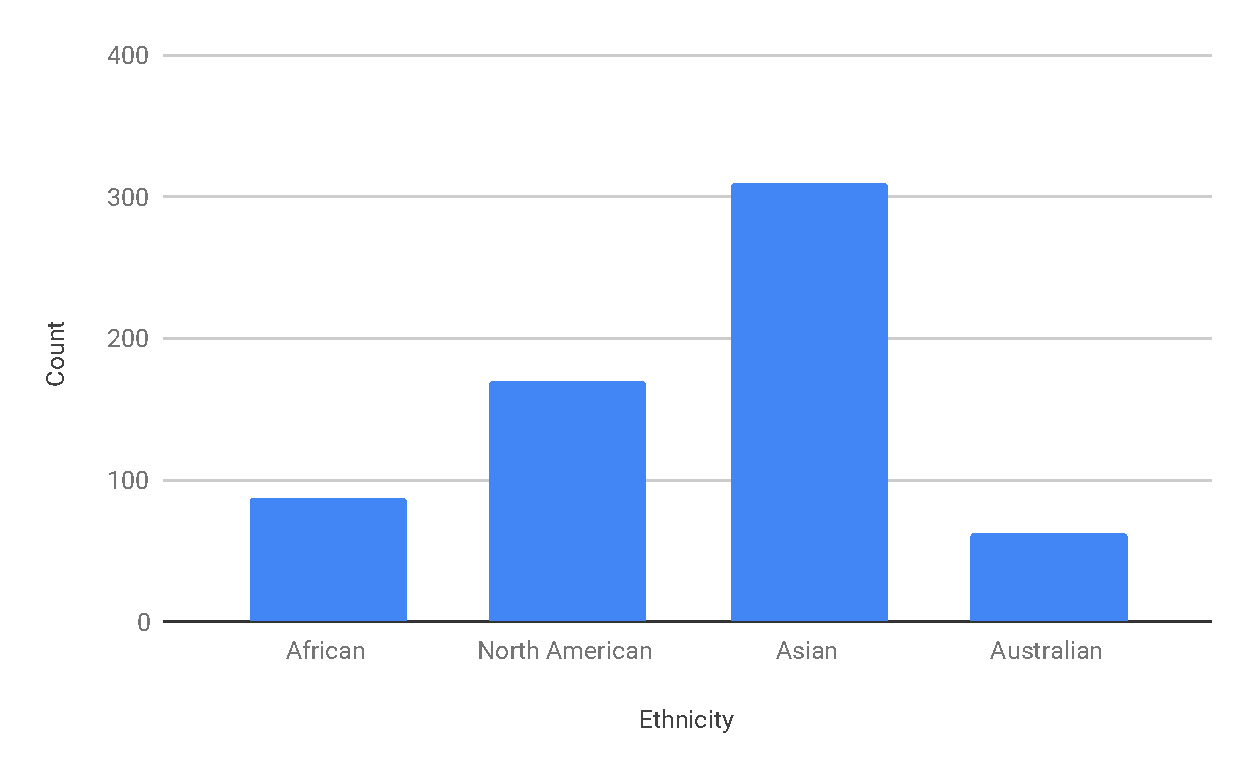
\includegraphics[width=\textwidth]{p-e.pdf}
    \caption{Ethnicity of participants}
    \label{fig:figone}
\end{figure}

\begin{figure}[hbtp]
    \centering
    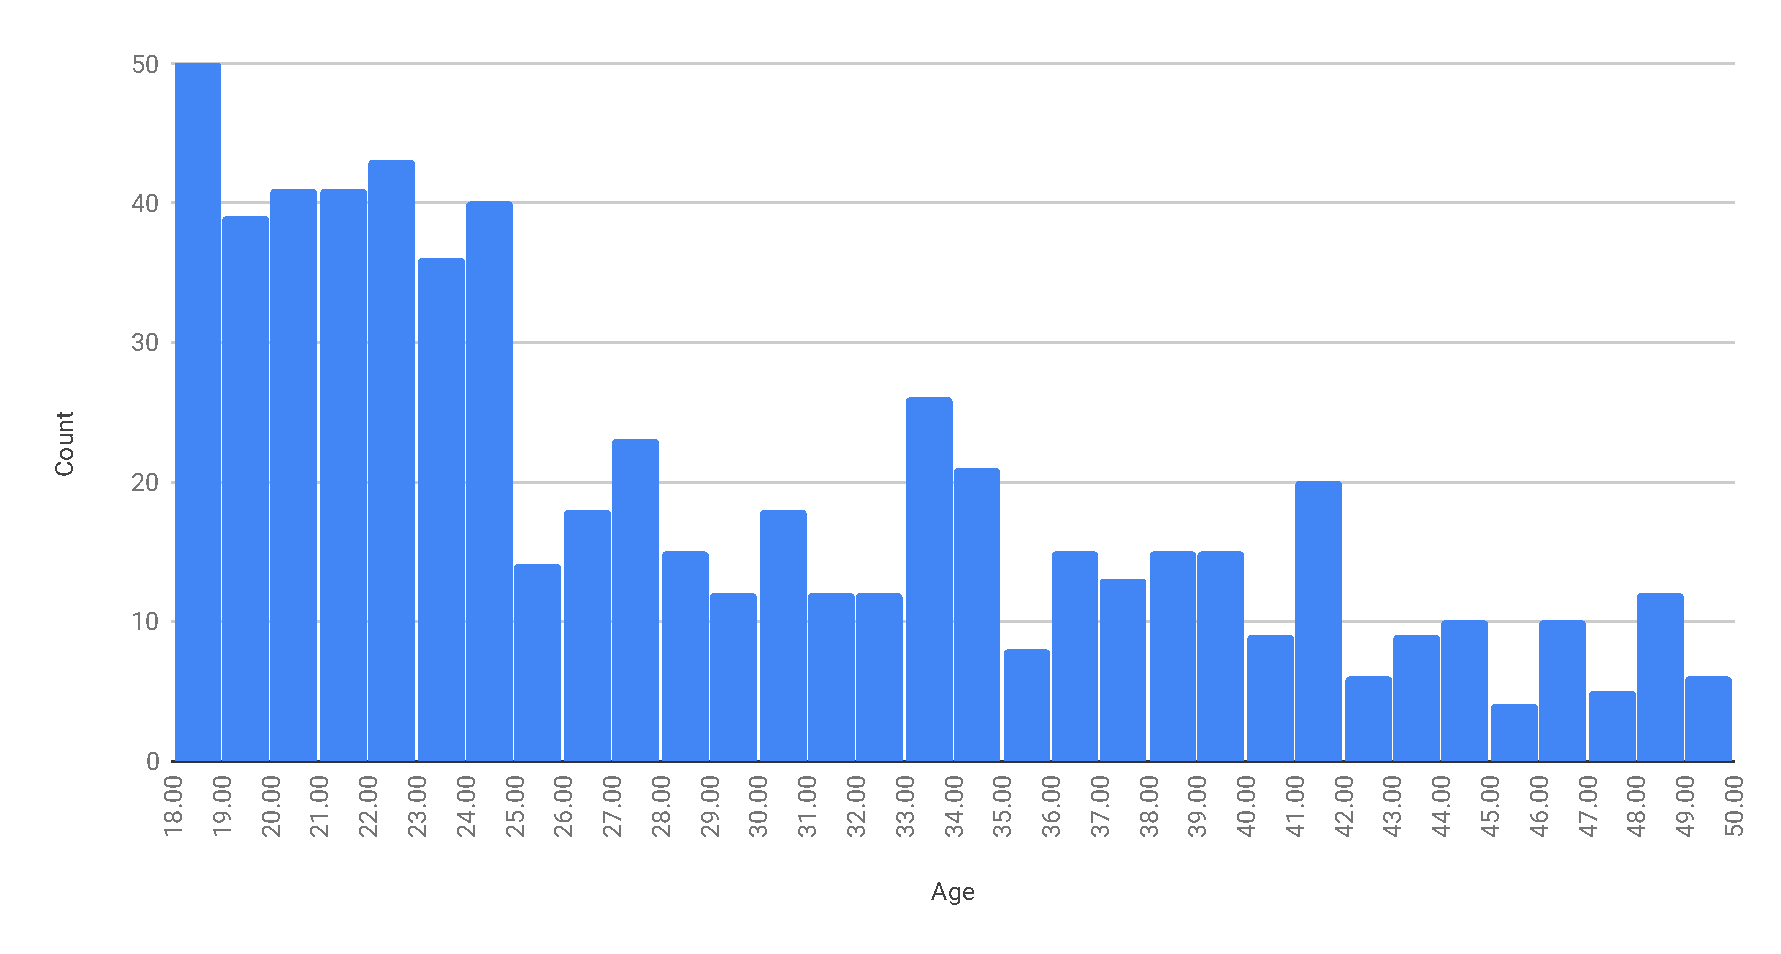
\includegraphics[width=\textwidth]{p-a.pdf}
    \caption{Age of participants}
    \label{fig:figtwo}
\end{figure}

\begin{figure}[hbtp]
    \centering
    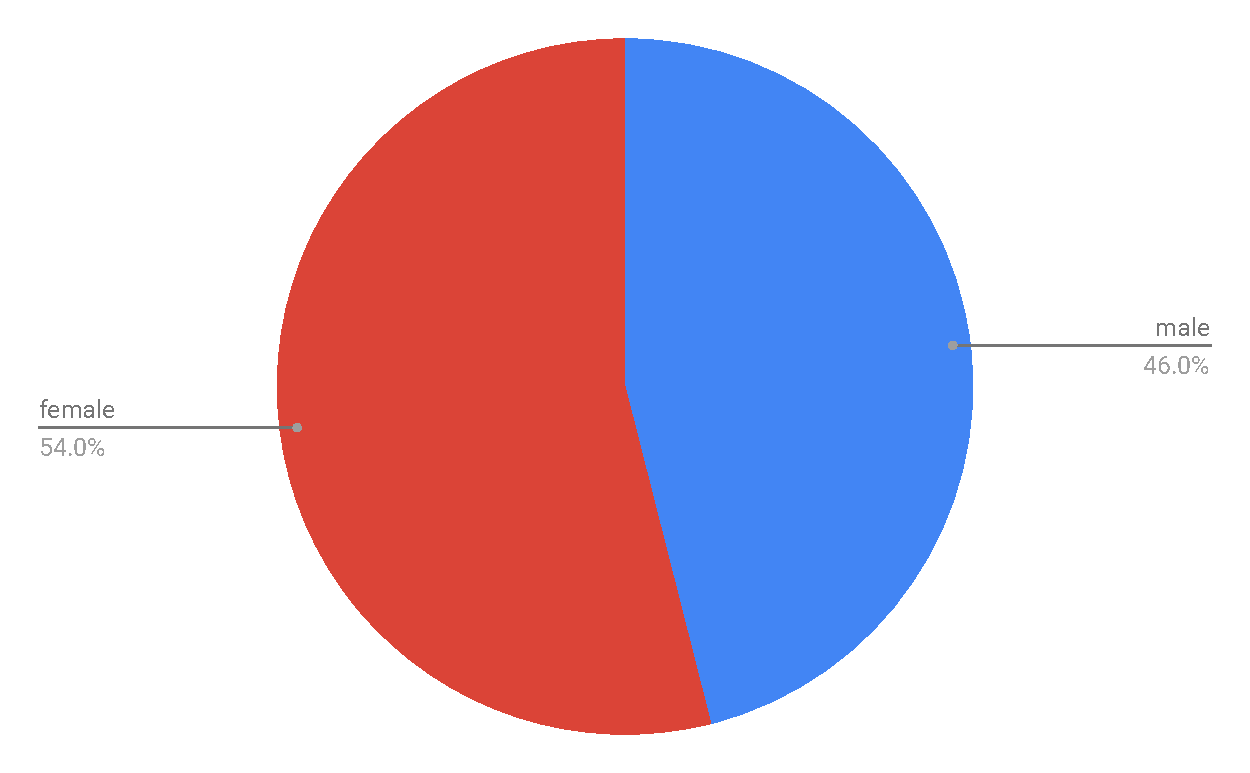
\includegraphics[width=\textwidth]{p-g.pdf}
    \caption{Gender of participants}
    \label{fig:figthree}
\end{figure}

\subsubsection{Data collection}

\paragraph{} We mentioned earlier that three kinds of data are collected from each user, and all these data are collected on a temporal (day-to-day) basis, and this is collected in such a manner so that a timeline of brain-wave data can be generated, which can be backed by usage patterns which are inferred from eye movement data and touchscreen interaction data. Thus, we take five points of analysis for each smartphone user:

\begin{itemize}
    \item the variation in the five kinds of brain waves (alpha, beta, gamma, delta and theta),
    \item the variation in frequency and speed of eye movements,
    \item the usage patterns (inferred from touchscreen interaction data and eye movement data),
    \item the exact time of usage across each day,
\end{itemize}

\paragraph{} all of which were plotted over the duration of the whole experiment. The results were pooled together into groups according to which group each participant belonged to, and then they were collated together, accounting for variance (with general standard deviation functions) and then the collated results of each group were compared against one another to obtain the final results, which would be the instrumental data that would then prove/disprove the hypothesis.

\subsubsection{Results and Discussion}

\paragraph{} The experiment's results are discussed from the two main types of data that was collected from the participants i.e. the brain-wave data and the eye movement data. The touchscreen interaction pattern data has only been used to confirm the active usage of the device when the screen of the smartphone is turned on, the absence of which implies that the user is inactive or watching content, which can be confirmed with the foreground application that the device is running. 
\begin{table}[hbtp]
  \begin{center}
    \begin{tabular}{|l|c|c|}
    \hline
                         & \multicolumn{2}{c|}{\textbf{Average usage (in hours)}}      \\ \hline
    \textbf{Group}       & \textbf{Before limiting}        & \textbf{After limiting}   \\ \hline
    Control group        & 6.72                   & 6.72                               \\ \hline
    First variant group  & 6.91                   & 4.71                               \\ \hline
    Second variant group & 6.45                   & 1.89                               \\ \hline
    \end{tabular}
    \caption{Comparison of usage (in hours) before and after limiting usage}
    \label{tab:tabone}
  \end{center}
\end{table}


\paragraph{} \textbf{Eye movement data}: We recorded the data of the participants and measured the frequency of eye movements over 10-second periods, which were then pooled together based on the group the user belonged to, and then the comparative analysis was made using data presented in Figure \ref{fig:res_eye_movement}. The decline in the average samples indicating slow eye movements (indicating lethargy and drowsiness) shows the decrease in lethargy felt in overall when the usage is restricted. The control group that has unrestricted access to their smartphones have the least active eye movement patterns. The first variant group that were restricted access to five hours per day shows a noticeable improvement in active eye-movement patterns. This improves even further with the second variant group who were restricted access to two hours per day. From this curve, it can be inferred that the users that are restricted usage to their smartphones refrain from using their smartphone in a compulsive manner and resort to using their smartphones in a relatively productive manner.

\begin{figure}[hbtp]
    \centering
    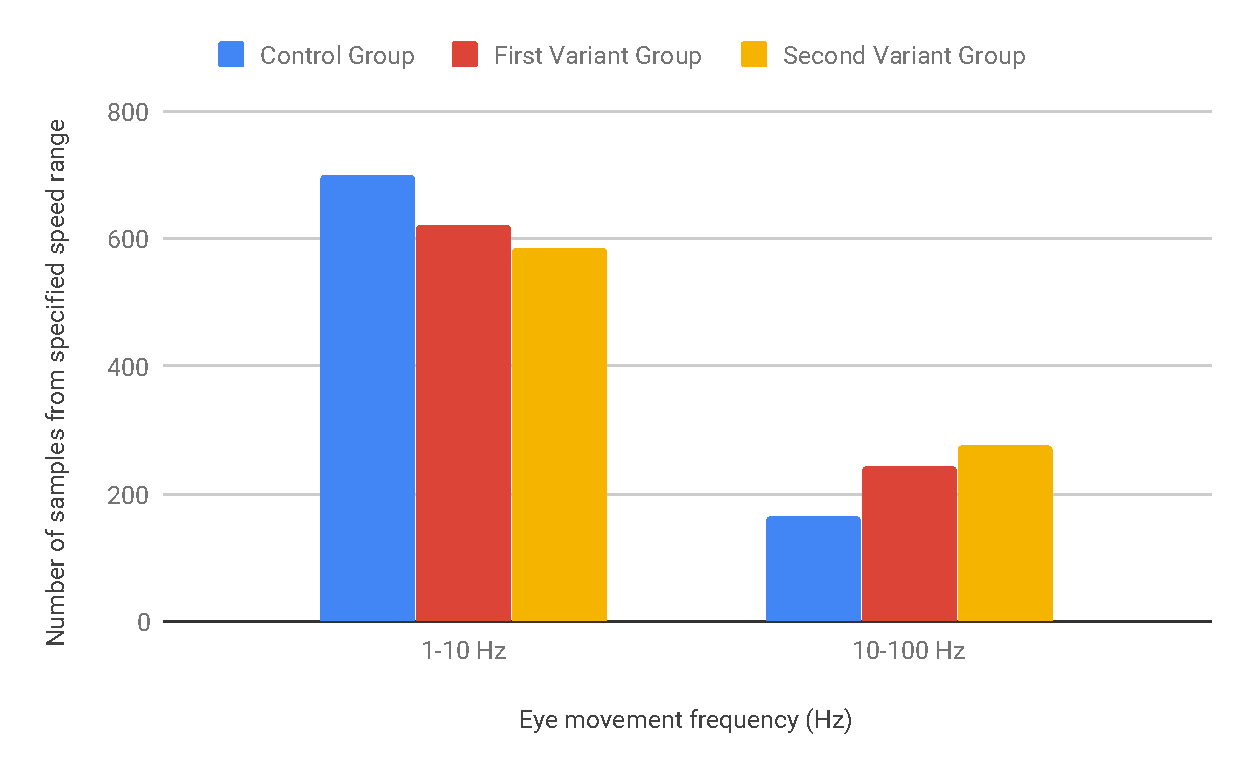
\includegraphics[width=\textwidth]{eye.pdf}
    \caption{Aggregate eye movement frequency per group}
    \label{fig:res_eye_movement}
\end{figure}

\paragraph{} \textbf{Brain-wave data}: We analyzed the brain-wave patterns of smartphone users over a period of 60 days, in which the analysis of the obtained data presented the percentages of each type of brain-wave, which in turn was used to infer the relative mental status of each group on an average. The brain-wave data indicated that the users when restricted access to their smartphones (shown by the first and second variant groups) show better REM (Rapid Eye Movement) sleep activity, which is an important factor in maintaining mental health. Moreover, there is a gradual increase in the percentage of gamma waves and beta waves, which imply that users are able to stay more focused on their current task without being susceptible to distractions. Another thing to note is that the proportions of alpha and delta waves even out, which means that the sleep patterns are also made proper even if REM sleep is not to be factored in. From this we can infer that the dreamless sleep and heavy sleep states of the users mind are equalized when the restrictions are imposed.

\begin{table}[htbp]
  \begin{center}
    \begin{tabular}{|rr|c|c|c|}
      \hline
      \multicolumn{1}{|l}{}       & \multicolumn{1}{l|}{} & \multicolumn{3}{c|}{Group}               \\ \cline{3-5} 
                                  & \multicolumn{1}{c|}{} & Control & First variant & Second variant \\ \hline
      \multicolumn{1}{|r|}{}      & Alpha waves           & 20      & 24            & 18             \\ \cline{2-5} 
      \multicolumn{1}{|r|}{\%}    & Beta waves            & 20      & 26            & 30             \\ \cline{2-5} 
      \multicolumn{1}{|r|}{of}    & Gamma waves           & 5       & 6             & 8              \\ \cline{2-5} 
      \multicolumn{1}{|r|}{waves} & Delta waves           & 35      & 30            & 19             \\ \cline{2-5} 
      \multicolumn{1}{|r|}{}      & Theta waves           & 20      & 22            & 25             \\ \hline
    \end{tabular}
    \caption{Average percentages of brain waves of users of each group}
    \label{tab:tabtwo}
  \end{center}
\end{table}

\subsection{Experiment 2 : Testing efficiency of solution}

\paragraph{} To analyze the effectiveness of SageSense, we propose an experiment that tests the variation in mental health levels of smartphone users that use SageSense. The experiment will provide an insight into the measure of how effective the solution is in reducing excessive and/or compulsive usage of smartphones. To conduct this experiment, we run an analysis of brain-wave patterns recorded at two points in time; at the beginning of the experiment before the user starts to use SageSense, and at the completion of the experiment, which is the mark at which the user completes 60 days of its continued usage. This data is recorded at both points for a 24-hour frame, to gain clearer knowledge into the user's day-to-day usage patterns before and after using SageSense.


\subsubsection{Research Data}

\paragraph{} The experiment attempts to contrast the states of mental health the participants are in before they start using SageSense with that at the completion of the duration of the experiment i.e. 60 days. This is performed by recording brain-wave patterns of the participants for a 24-hour period at both specified points in time. The brain-wave data collected include levels of five types of brain waves, namely alpha waves, beta waves, gamma waves, delta waves and theta waves. This requires the participants to complete 60 days of continued usage of SageSense, failing which will render the participant's data invalid for the experiment. We utilize the guidelines that were formulated in our first experiment to analyse the trends/patterns in the recorded brain-wave data.

\subsubsection{Experimental Setup}

\paragraph{} We are measuring the effectiveness of SageSense and as such, the major component of the experimental setup is SageSense itself. It's method of collection of brain-wave data allows us to aggregate the data from the participants of the experiment. SageSense's wearable headband records brain-wave data in real-time and sends it to the application which locally processes the data on the smartphone itself, which then provides dynamic lockout timeframes to the user. In this experiment, however, we use a modified version of SageSense that sends the recorded data to our central database hosted on a data collection server. This acts as the central source of data. The data is collected from each participant two times over the whole duration of the experiment; at the beginning of the experiment and at the end of the experiment. These instances of data collection are done with each participant for a continuous 24-hour time period, to measure the usage of the phone and the brain-wave activity of the user over the course of a whole day.

\subsubsection{Research Design}

\paragraph{} The experiment was conducted on a multi-ethnic group of 500 participants (Ethnicity: 20\% North American, 45\% Asian, 25\% African and 10\% Australian; Gender: 51\% male, 49\% female; Age: 18-24 - 37\%, 25-40 - 41\%, 41-50 - 22\%). These participants were divided into two groups on the criteria that each group consisted of an equal number of participants whose usage when taken on an average should roughly equal (allowing tolerance of +/-0.5 hours) that of the other group. The first group became the control group, which consisted of 250 participants and the second group became the variant group, which consisted of 250 participants. 

\paragraph{} Since we aim to test the effectiveness of SageSense, we utilize the same to record the brain-wave activity of each participant over two 24-hour periods over the duration of the experiment (start and end of the experiment) whilst he/she is using the wearables that provide SageSense with its data. This will provide data on the brain-wave patterns of the five kinds of brain waves that we record with SageSense i.e. alpha, beta, gamma, delta and theta waves. 

\paragraph{} Participants of the control group are not given the chance to use SageSense's ability to deliver lockout timeframes, and are allowed unrestricted access. However, participants of the variant group have this ability enabled, effectively restricting the usage of their smartphones over the duration of the experiment (60 days).

\subsubsection{Data Collection}

\paragraph{} We collect brain-wave activity of each participant at two points in time; at the start of the experiment and at the end of the experiment. Each instance of data collection is run for 24 hours to get the complete data of brain-wave activity of a user over a whole day. SageSense records five kinds of brain-waves (alpha, beta, gamma, delta, theta) which are used as the datasets to compare the brain-wave patterns amongst the two instances of brain-wave data collection (the start of the experiment and the end of the experiment). We finally compare the data obtained from the control group and the variant group to measure the approximate measure of effectiveness of SageSense amongst the userbase.


\clearpage
\bibliographystyle{plainnat}
\bibliography{cite}

\end{document}